% ------------------------------------------------------------------------------
% Revisão Bibliográfica
% ------------------------------------------------------------------------------

\chapter{Revisão Bibliográfica}\label{chap:revisao}

\section{Ciclo de Vida}\label{sec:revisao:ciclodevida}

	A definição e criação de um ciclo de vida é uma das formas da Engenharia de Sistemas (ES) atuar no seu propósito de viabilizar o sucesso de um sistema ao
	mesmo tempo que otimiza a competição existente entre os objetivos das partes interessadas. Ao desmembrar o esforço total e definir os estágios, seus papéis, as novas características do sistema, os critérios de conclusão, os riscos envolvidos e, finalmente, tomar uma decisão, está-se criando o ciclo de vida. Esse processo organiza e estrutura as etapas necessárias para o desenvolvimento e a evolução do sistema de forma clara e eficiente.

	Entre cada estágio definido, existem os chamados \textit{decision gates} (portões de decisão, em tradução livre). Nesses pontos, é realizada uma análise do progresso e, como o nome sugere, uma decisão é tomada em relação ao desenvolvimento do sistema.

	O ciclo de vida de um sistema é definido a partir de suas características e particularidades, de modo que seus estágios sejam inseridos para atender todas as suas
	necessidades. Os estágios podem aparecer mais de uma vez, serem executados sequencialmente ou paralelamente e serem inseridos a qualquer momento do ciclo de vida.

	Em alguns casos, o Sistema de Interesse (SoI, do inglês \textit{System of Interest}) faz parte de um Sistema de Sistemas (SoS, do inglês \textit{System of Systems}). Nesse contexto, cada um possui seu próprio ciclo de vida. Geralmente, em um SoS, cada elemento do sistema tem seu ciclo de vida independente, e o ciclo de vida do SoS influencia diretamente o do SoI. Por isso, ao analisar o ciclo de vida do SoI, é essencial considerar a evolução e as interações com o SoS.

	O ciclo de vida genérico trazido no \cite{incoseHandbook} nos mostra os seis estágios básicos existentes numa estruturação em ``V'' que busca mostrar de forma visual a aparição desses estágios
	ao longo do tempo, realçando também o possível paralelismo entre eles. Os estágios são de: conceito, desenvolvimento, produção, utilização, suporte e descontinuação. Na figura \ref{fig:revisao:veeLifeCycle} podemos ver uma representação do que foi mostrado no livro. A seguir cada estágio será abordado:

	\begin{figure}[h]
		\centering
		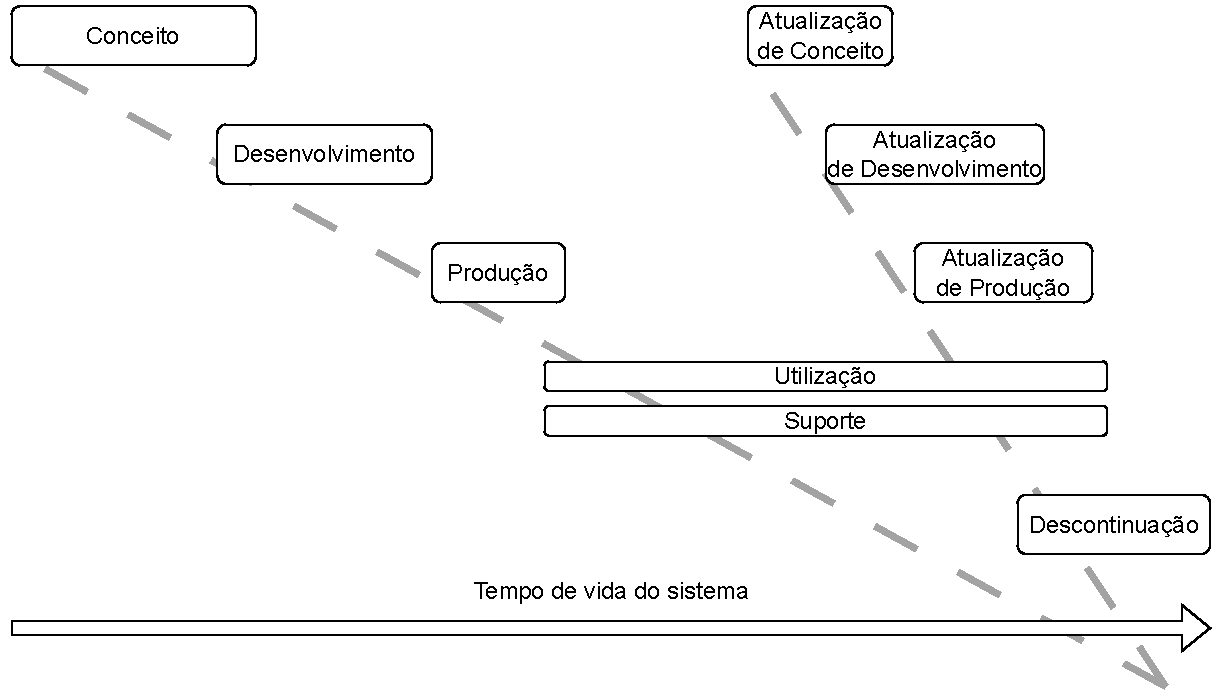
\includegraphics[width=\textwidth]{./figuras/veeLifeCycle.pdf}
		\caption{Ciclo de vida com estrutura em ``V''.}
		\label{fig:revisao:veeLifeCycle}
	\end{figure}

	\begin{itemize}
		\item Estágio de conceito: Este estágio representa a fase exploratória, onde são identificadas as origens de uma necessidade, uma nova missão, uma nova capacidade de negócio ou a alteração de algum desses elementos. Nele, são analisados diversos fatores do sistema, como mercado, aspectos ambientais, condições econômicas, recursos disponíveis e escopo de atuação. O objetivo é definir os limites do problema a ser resolvido, as missões do sistema, onde ele será aplicado e realizar uma análise do negócio, da missão e dos valores que serão entregues. Para garantir uma definição clara do problema, são realizados levantamentos dos requisitos do sistema, das partes interessadas envolvidas e de suas necessidades, além da exploração do espaço de soluções possíveis. Com base nisso, é possível estimar um custo inicial do esforço necessário e criar uma agenda preliminar, que servirá como base para o ciclo de vida do sistema. Alguns dos resultados típicos desse estágio incluem documentos preliminares da arquitetura do sistema, análise de viabilidade, requisitos, design, agenda e estimativa de esforço. Esse estágio é crucial, pois é nele que o sistema é definido. Embora mudanças possam ocorrer posteriormente, sua implementação tende a ser mais complexa e custosa devido a fatores como tempo e recursos adicionais necessários.
		\item Estágio de desenvolvimento: nesse estágio é definido um SoI que atende e vai de encontro com as necessidades e requisitos das partes interessadas, e que pode ser produzido, utilizado, suportado e descontinuado caso necessário. O objetivo principal dessa fase é definir um projeto base de engenharia que pode ser executado, sem buscar a perfeição, mas atendendo às partes interessadas e respeitando os possíveis ``trade-offs'' previamente definidos nesse mesmo estágio. Nesse projeto base devem estar os requisitos, arquitetura, modelagens, documentação e planejamento para próximas fases que também podem ser vistos como saídas dessa fazer.
		\item Estágio de produção: nesse estágio o projeto base definido no estágio de desenvolvimento, é aprovado e qualificado para ser colocado para utilização. Esse estágio simboliza o período de instalação, implementação ou transição para um ambiente de fato produtivo.
		\item Estágio de utilização: o início desse estágio se dá com a liberação do sistema ou parte dele para uso, incluindo os sistemas de apoio que são necessários para certas funcionalidades. Esse estágio comumente é o mais longo do ciclo de vida e é comum que mudanças e melhorias no SoI ocorram ao longo da utilização, lembrando sempre de fazer o gerenciamento dos riscos e documentação para garantir a integridade e manutenção do SoI.
		\item Estágio de suporte: segue paralelo ao estágio de utilização assim que alguma funcionalidade se torna disponível, no entanto o preparo e 
		planejamento desse estágio pode ser iniciado antes como a aquisição de sobresalentes. Nesse estágio que são percebidas as melhorias e mudanças que 
		podem vir a ser implementadas durante a utilização.
		\item Estágio de descontinuação: ocorre quando o sistema é retirado de operação, marcando o fim dos estágios de utilização e produção, ou, no máximo, 
		havendo uma pequena sobreposição entre eles. Além de definir como será realizado o descarte ou armazenamento físico ou virtual dos componentes do sistema, essa etapa 
		também envolve a análise da possível extensão da vida útil de algumas partes do sistema e o arquivamento de documentos importantes relacionados a ele.
		É uma fase crucial para garantir o encerramento adequado do ciclo de vida do sistema.
	\end{itemize}
	
	Ainda no \cite{incoseHandbook}, são trazidos conceitos importante sobre os \textit{decision gates} que coexistem entre os estágio dos ciclo de vida, tanto no início quanto no fim de cada estágio.
	Dentre os objetivos dos \textit{decision gates} estão o acompanhamento da evolução da maturidade do sistema, a conferência dos critérios de saída ou entrada de um estágio,
	a análise de risco mediante à situação atual do sistema, e por fim uma tomada de decisão sobre o que será feito. Podendo haver um regresso no ciclo de vida, um avanço, uma pausa 
	ou até mesmo o cancelamento do projeto.

	É importante saber equilibrar a formalidade e frequência desses eventos, visto que eles envolvem diferentes partes interessadas, gestores e especialistas, e além disso as
	decisões devem ser guiadas por dados tomados nos estágios do ciclo de vida e nos artefatos que são gerados para esse momento. Isso evita considerações desnecessárias e 
	inadequadas que podem prejudicar futuramente.

	As três abordagens principais trazidas pelo livro para os ciclos de vida são, sequencial, incremental e evolucionário. As principais características dessas três abordagens
	podem ser resumidas na tabela \ref{tab:revisao:ciclodevida:abordagens} apresentada.

	\begin{table}[!h]
		\centering
		\caption{Características das abordagens de um ciclo de vida}
		\begin{tabular}{cccc}
			\hline
			Abordagem & Requisitos definidos no ínicio & Iterações planejadas & Múltiplas instalações \\
			\hline
			Sequencial & Todos os requisitos & Apenas uma & Não\\
			Incremental & Todos os requisitos & Múltiplas & Potencialemnte\\
			Evolucionário & Parte dos requisitos & Múltiplas & Tipicamente\\
			\hline
		\end{tabular}
		\label{tab:revisao:ciclodevida:abordagens}
	\end{table}

	Durante a execução dos estágios do ciclo de vida várias tarefas são executadas, e para isso alguns processos precisam ser realizados para garantir a consistência das atividades. Um conjunto
	de processos é definido no livro e a execução de cada um deles varia de acordo com os estágios existentes no ciclo de vida do sistema.

	\subsection{Fases dos estágios de Conceito e Desenvolvimento}\label{sec:revisao:ciclodevida:fases}

	\cite{kossiakoff2020systems} fazem uma quebra dos estágios de conceito e desenvolvimento citados anteriomente, subdividindo-os em três fases cada. Dessa maneira a análise do ciclo de vida
	de um sistemas, bem como a sua estruturação fica mais clara e objetiva.
	Para o estágio de conceito temos as fases mostradas na figura \ref{fig:revisao:conceptStagePhases}, \cite{kossiakoff2020systems} as descreve da segunte maneira:
	
	\begin{figure}[h]
		\centering
		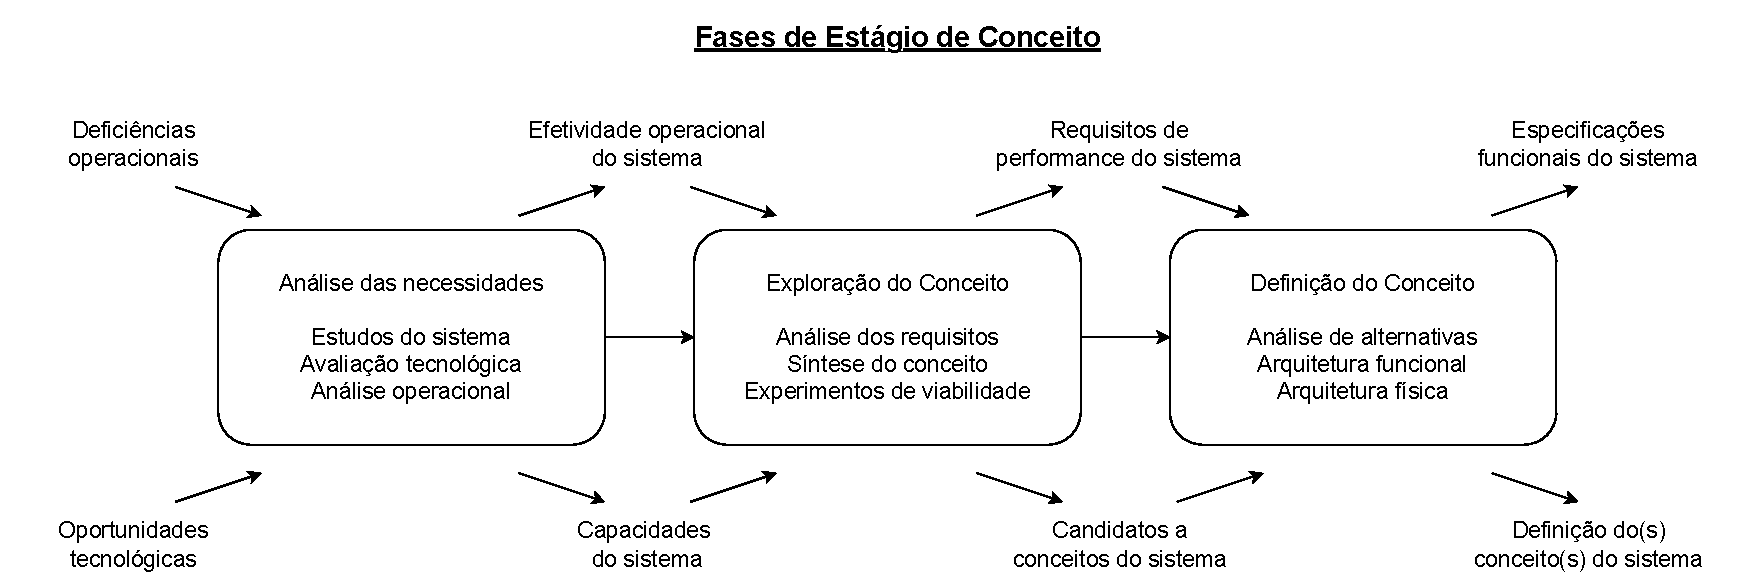
\includegraphics[width=\textwidth]{./figuras/conceptPhases.pdf}
		\caption{Fases do estágio de Conceito, adaptado de \citep{kossiakoff2020systems}}
		\label{fig:revisao:conceptStagePhases}
	\end{figure}

	\subsubsection*{Fase de análise de necessidade}
	 
	A fase de análise de necessidades tem como objetivo identificar se há, de fato, uma necessidade legítima para o desenvolvimento de um novo sistema, bem como 
	avaliar se existe uma abordagem viável para atendê-la. Essa etapa exige uma análise crítica das limitações dos meios existentes em
	suprir as demandas atuais ou futuras previstas. Também é considerada a viabilidade técnica, ou seja, se a tecnologia disponível é capaz de suportar a 
	capacidade adicional desejada.
	
	Frequentemente, o início do ciclo de vida de um sistema não se dá de forma repentina, mas sim como resultado de uma análise contínua das necessidades 
	operacionais ou do desenvolvimento de produtos inovadores. O principal resultado dessa fase é a descrição das capacidades e da efetividade operacional 
	esperadas do novo sistema. Embora ainda não configure um conjunto formal de requisitos, essa 
	descrição serve como base para sua futura definição.
		
	Para apoiar essa fase, são utilizados diversos métodos e ferramentas, especialmente as áreas da análise operacional e da pesquisa operacional. Além disso, 
	avaliações tecnológicas e experimentações complementam essas abordagens matemáticas, contribuindo para uma definição mais precisa das necessidades do sistema.

	\subsubsection*{Fase de exploração de conceito}

	Na fase de exploração de conceitos, busca-se responder às seguintes questões: “Qual desempenho o novo sistema precisa atingir para satisfazer a necessidade 
	identificada?” e “Existe pelo menos uma abordagem viável para alcançar esse desempenho a um custo aceitável?” A resposta positiva a essas perguntas é essencial 
	para estabelecer objetivos realistas e viáveis antes de investir fortemente no desenvolvimento do sistema.

	O principal resultado desta fase é a formulação do primeiro conjunto de requisitos de desempenho do sistema, considerados “oficiais” por serem passíveis de 
	medição e avaliação por parte de contratantes ou agências. Além disso, são gerados os conceitos candidatos de sistema — ou seja, múltiplas alternativas de 
	solução. A exploração de diferentes abordagens é fundamental para compreender as possibilidades disponíveis para atender à necessidade identificada.

	Diversas ferramentas e técnicas são utilizadas nessa etapa, incluindo métodos de processo (como análise de requisitos) e julgamento especializado 
	(como sessões de brainstorming). Inicialmente, o número de conceitos pode ser elevado, mas o processo visa reduzi-los 
	rapidamente a um conjunto manejável. A viabilidade das alternativas finais precisa ser comprovada, pois elas serão a base para as decisões da próxima fase do 
	ciclo de vida.
	
	\subsubsection*{Fase de definição de conceito}

	A fase de definição de conceito tem como foco selecionar o conceito de sistema mais promissor, ou seja, aquele que apresenta o melhor equilíbrio entre 
	capacidade, vida útil operacional e custo. Para isso, diferentes alternativas devem ser comparadas em relação ao desempenho, utilidade operacional, riscos 
	de desenvolvimento e custos. Com base nessa análise, é decidido se vale a pena investir recursos significativos no desenvolvimento do novo sistema.

	O principal resultado dessa fase é uma descrição funcional clara do que o sistema deve fazer e qual desempenho deve alcançar, além da definição do conceito 
	selecionado de sistema. Em sistemas simples, essa descrição pode ser feita de forma direta; em sistemas mais complexos, é necessária uma arquitetura de sistema 
	mais detalhada, que represente o sistema sob diferentes perspectivas — principalmente funcional e física.

	As ferramentas utilizadas nesse estágio incluem análise de alternativas e práticas de arquitetura de sistemas. Em contextos comerciais, as 
	fases anteriores são frequentemente integradas em um estudo de viabilidade, que serve como base para decidir se o conceito deve ser desenvolvido.

	Mesmo que já tenham sido dedicados esforços significativos na compreensão do ambiente operacional e das tecnologias relacionadas, até este ponto o 
	investimento direto no desenvolvimento do sistema costuma ser limitado. É nas fases seguintes que a maior parte dos recursos será aplicada, com foco no 
	desenvolvimento técnico e implementação.

	Olhando agora para o estágio de desenvolvimento vemos na figura \ref{fig:revisao:developmentStagePhases} suas fases e entradas e saídas. Novamente suas definições segundo \cite{kossiakoff2020systems} encontram-se abaixo:

	\begin{figure}[h]
		\centering
		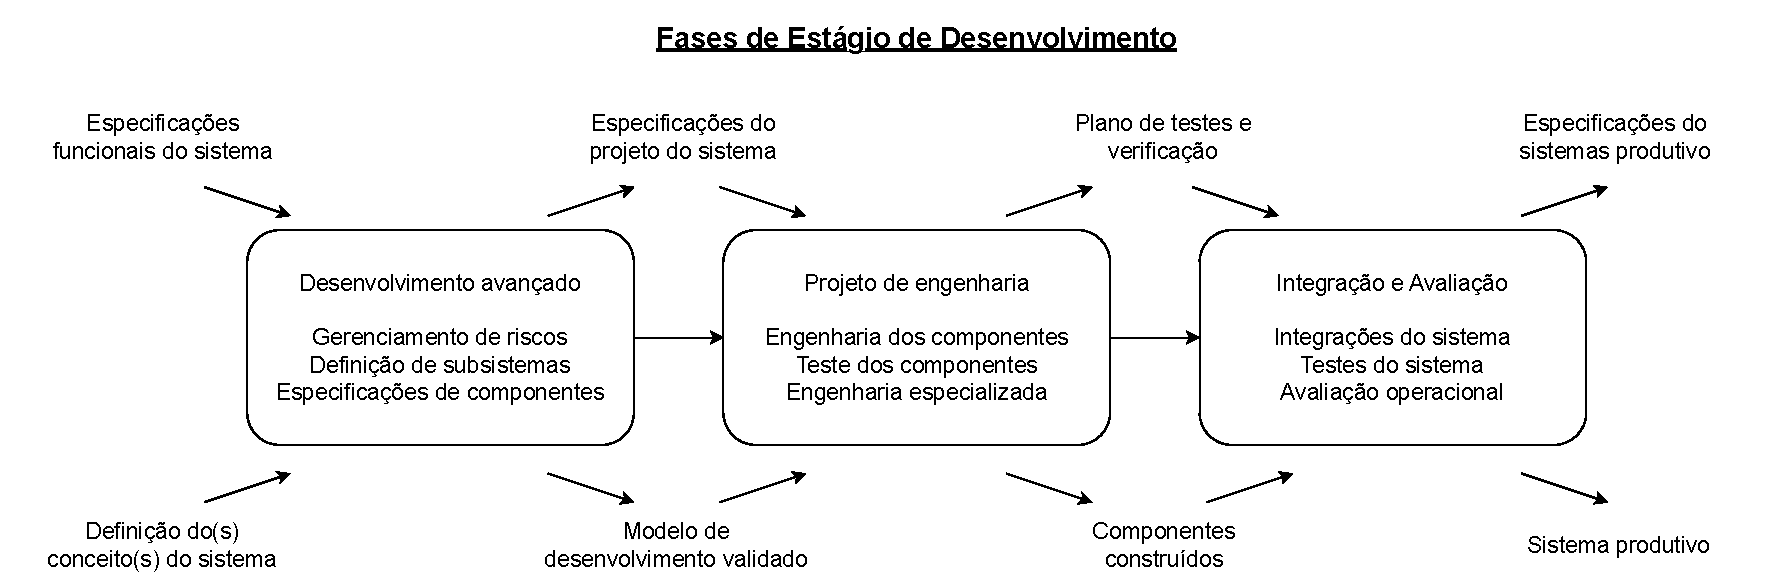
\includegraphics[width=\textwidth]{./figuras/developmentPhases.pdf}
		\caption{Fases do estágio de Desenvolvimento, adaptado de \citep{kossiakoff2020systems}}
		\label{fig:revisao:developmentStagePhases}
	\end{figure}

	\subsubsection*{Fase de desenvolvimento avançado}
	A fase de desenvolvimento avançado marca a transição entre a definição conceitual e o início do desenvolvimento técnico de um sistema. Seu sucesso depende 
	fortemente da solidez das decisões tomadas nas fases conceituais anteriores. No entanto, como essas fases iniciais geralmente envolvem análises com recursos 
	limitados, ainda restam incertezas importantes que precisam ser identificadas e resolvidas o quanto antes. Esta fase tem como principal objetivo minimizar 
	esses riscos e transformar os requisitos funcionais do sistema em especificações técnicas mais detalhadas.

	Duas finalidades centrais definem esta fase: a identificação e mitigação de riscos de desenvolvimento, e a produção das especificações de design do sistema. 
	Isso é particularmente crítico em projetos que envolvem tecnologias inovadoras ou desempenho que extrapola os limites previamente testados. A fase 
	concentra-se no desenvolvimento e validação das partes do sistema que ainda não estão consolidadas, assegurando que seus requisitos possam de fato ser 
	atendidos.

	Nesta etapa, a ES desempenha papel essencial ao definir o que precisa ser validado, como isso será feito e como interpretar os resultados 
	obtidos. Frequentemente, modelos experimentais e simulações são empregados para validar conceitos de projeto de componentes e subsistemas, reduzindo os custos 
	de desenvolvimento.

	O produto final desta fase é um modelo de desenvolvimento validado, junto a um conjunto refinado de especificações de projeto. Esse modelo deve demonstrar que
	o sistema pode ser projetado e fabricado de forma viável e com riscos aceitáveis. Por isso, todos os riscos precisam estar classificados como controláveis 
	antes que o projeto avance para a próxima fase do ciclo de vida.

	\subsubsection*{Fase de projeto de engenharia}

	A fase de projeto de engenharia representa a transição entre a definição conceitual e a concretização técnica do sistema. É nesta etapa que o projeto detalhado 
	dos componentes é desenvolvido, resultando na criação de um protótipo funcional ou virtual do sistema. Devido à sua complexidade e escopo, essa fase é geralmente
	marcada por revisões formais de projeto, que permitem ao cliente acompanhar o progresso, controlar custos, revisar o cronograma e fornecer feedback essencial 
	aos desenvolvedores.

	Embora aspectos como confiabilidade, manutenibilidade e fabricabilidade – conhecidos como ``Engenharia especializada'' – já tenham sido considerados anteriormente, 
	nesta fase eles assumem um papel central. O engenheiro de sistemas tem a responsabilidade de garantir que cada componente implementa corretamente os requisitos 
	funcionais e de compatibilidade, além de coordenar o processo de mudanças de engenharia para manter o controle das interfaces e da configuração do sistema.

	As principais atividades dessa etapa incluem a conversão das especificações de componentes em projetos de engenharia completos, além da execução de testes 
	preliminares. Esses testes podem ser realizados imediatamente após o projeto ou paralelamente a ele. Outro elemento crucial é o refinamento do plano de testes e 
	avaliações (T\&A), iniciado em fases anteriores, mas consolidado com base nas decisões e dados acumulados até aqui.

	Os dois principais produtos desta fase são o plano de T\&A e um protótipo do sistema. Este protótipo pode assumir diferentes formas — física, virtual ou híbrida — 
	dependendo da natureza do sistema em questão. Por exemplo, no caso de sistemas complexos e de grande escala, como embarcações de carga, o protótipo pode combinar
	simulações digitais e modelos físicos em escala reduzida.

	Ferramentas modernas de projeto assistido por computador (CAD) e simulações de sistemas são amplamente utilizadas para apoiar as decisões de engenharia, 
	garantindo que o sistema projetado seja viável, testável e alinhado com os objetivos operacionais definidos nas fases iniciais do ciclo de vida.

	\subsubsection*{Fase de integração e avaliação}
	A fase de integração e avaliação marca o momento em que os componentes projetados e desenvolvidos são reunidos para formar um sistema funcional completo. 
	Embora ainda seja parte do processo de desenvolvimento, essa etapa possui características distintas, especialmente no que diz respeito ao papel da ES, 
	justificando seu tratamento como uma fase separada no ciclo de vida do sistema.

	É nessa etapa que o sistema é montado e testado pela primeira vez em um ambiente realista ou simulado. Isso permite verificar se as interfaces entre os 
	componentes estão compatíveis e se a integração geral atende aos requisitos funcionais estabelecidos. Apesar de testes prévios em subsistemas ou protótipos 
	terem sido realizados, somente agora é possível validar a integridade do sistema como um todo.

	Frequentemente, a execução dessa fase exige a construção de instalações específicas capazes de simular estímulos operacionais e restrições reais, de modo a 
	permitir uma avaliação precisa do desempenho do sistema. A complexidade e os recursos necessários para essa infraestrutura não devem ser subestimados.

	Os principais resultados da fase de integração e avaliação são: (i) as especificações finais de produção do sistema, conhecidas como ``baseline de produção'', 
	que orientam a fabricação do produto final, e (ii) o sistema de produção propriamente dito, que inclui tudo o que é necessário para manufaturar e montar o 
	sistema em escala.

	Ferramentas modernas de integração, T\&A, bem como métodos e princípios atualizados, estão disponíveis para apoiar os engenheiros nesse processo. Antes que a 
	produção em larga escala possa começar, é essencial que o sistema final seja verificado e validado em um ambiente operacional real ou em uma simulação que represente 
	fielmente esse contexto.

	\vspace{1.5 cm} % Precisa desse espaçamento?
	
	\cite{kossiakoff2020systems} trazem ainda um relacionamento entre as fases desses dois estágios com os níveis de detalhamento do sistema. De maneira visual é destacado
	em quais os níveis cada fase deve alcançar, consequentemente definindo o detalhamento de cada fase. Assim fica mais claro a materialização do sistema, onde as primeiras fases tocam
	na parte mais superficial e mais abstrata, e a medida que se avança de fase, vai se adentrando nos níveis de funcionalidades, quebrando e detalhando as funções e associando-as com
	os elementos do sistema no nível correspondente. A tabela \ref{tab:revisao:systemMaterialization} ilustra essas relações.


	É fundamental perceber que, mesmo que o projeto detalhado só se conclua tardiamente no
	desenvolvimento, a visualização geral do sistema deve ocorrer ainda nas fases iniciais.
	Isso é necessário para estimar custos, viabilidade técnica e orientar a escolha do conceito do sistema.
	A visualização inicial não precisa ser precisa em todos os detalhes, mas deve ser realista o suficiente
	para orientar decisões viáveis.

	\begin{table}[H]
		\centering
		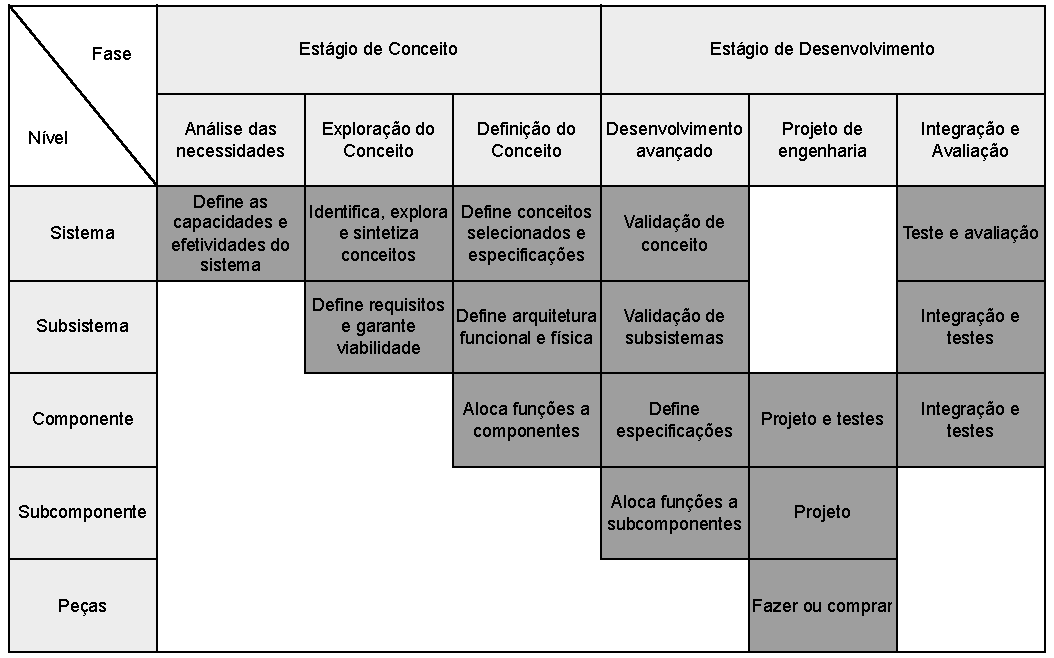
\includegraphics[width=\textwidth]{./figuras/systemMaterialization.pdf}
		\caption{Materialização do sistema, adaptado de \citep{kossiakoff2020systems}}
		\label{tab:revisao:systemMaterialization}
	\end{table}

	\subsection{Estágios de Pós Desenvolvimento}\label{sec:revisao:ciclodevida:posDev}
	Após a conclusão do desenvolvimento de um sistema, inicia-se a etapa pós-desenvolvimento, composta por duas fases principais, de acordo com
	\citep{kossiakoff2020systems}: Produção e Utilização e suporte. Os autores unificaram Utilização e Suporte pois de fato seguem em paralelo a todo momento.
	Porém, será adicionado o último estágio do ciclo de vida apresentado pelo \cite{incoseHandbook} a esse grupo, o estágio de Descontinuação. A figura
	\ref{fig:revisao:postDevelopment} trás no mesmo estilo a representação desses estágios.

	\begin{figure}[h]
		\centering
		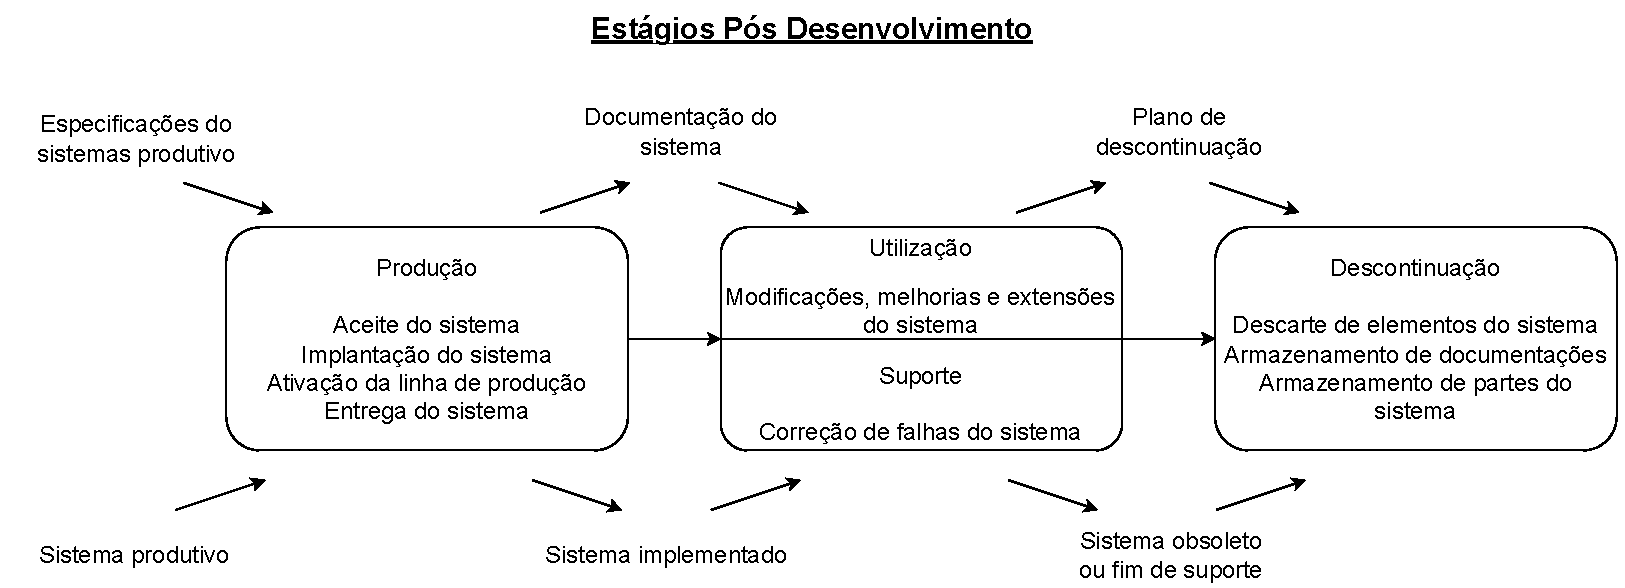
\includegraphics[width=\textwidth]{./figuras/postDevelopment.pdf}
		\caption{Estágio de Pós Desenvolvimento, adaptado de \citep{kossiakoff2020systems}}
		\label{fig:revisao:postDevelopment}
	\end{figure}
	
	\section{Arquitetura do Sistema}\label{sec:revisao:arqSistema}

	Como mencionado na seção \ref{sec:revisao:ciclodevida} existem diferentes etapas durante o ciclo de vida de
	um sistema. Uma delas é o ``Processo de Definição da Arquitetura do Sistema'', que tem como objetivo, conforme registrado
	no \cite{incoseHandbook}, gerar alternativas de arquiteturas do sistema, selecionar uma ou mais alternativa que atende aos
	requisitos das partes interessadas, e expressar isso em uma visualização e modelos consistentes.

	Dessa forma, esse processo provê informação e dados necessários para identificar e caracterizar os conceitos e
	propriedades fundamentais do sistema e seus elementos. Esse processo é vivo ao longo do ciclo de vida, e deve ser sempre
	retomado quando há modificações de conceitos ou de perspectivas no decorrer do desenvolvimento do sistema.

	Dentre as entradas para a execução desse processo mostradas no \cite{incoseHandbook}, destacam-se os ``Requisitos do Sistema'',
	as ``Restrições de solução'', a ``Descrição do projeto do sistema'', ``As soluções alternativas'' e um ``Projeto de arquitetura validado e verificado''.

	Com essa entradas em mãos são realizadas as atividades para a definição de qual será a arquitetura definitiva do sistema. E após
	isso temos como saídas resultantes típicas os ``Artefatos e registros da arquitetura do sistema definida'', a ``Descrição da 
	arquitetura do sistema'', o ``Mapeamento de rastreabilidade'' e a ``Justificativa da arquitetura do sistema''.
	 
	A existência de um ``Estilo de Arquitetura'' é de extrema importância para que esse processo seja executado com êxito.
	Ele	atua como um modelo, ou guia, para se construir a arquitetura do sistema. Os ``Estilos de Arquitetura'' podem 
	ser definidos com base nos ponto de vista da arquitetura, nos elementos do
	sistema e seus relacionamentos, nas conexões, interfaces, mecanismos de interação e possíveis restrições.
	
	Além dos ``Estilos de Arquitetura'', outro conceito importante é o de ``Padrões de Arquitetura''. 
	Eles são modelos simplificados mas completos no que diz respeito aos elementos do
	sistema e são reutilizáveis para diferentes tipos cenários. O uso de ``Padrões de Arquitetura'' agiliza  a 
	documentação, facilita a comunicação, promove o reúso, melhora a produtividade
	e eficiência e serve como um ponto de início para o desenvolvimento de novos sistemas.

	Como o conceito de arquitetura pode ser muito abrangente, o \cite{sebok2024} mostra três segmentações, a arquitetura funcional, lógica e a física.

	A arquitetura funcional compreende as funcionalidades do sistema, ou seja, quais funções ou comportamentos 
	aquele sistema executa ou possui em diferentes contextos para atingir os objetivos esperados pelos diferentes interessados.
	Essa arquitetura está fortemente conectada com a definição de conceito do sistema e tem papel chave em dar início à materializaçao do sistema
	ao traduzir esses conceitos em um projeto de sistema viável. Não há exatamente um modelo ou padrão recomendado de
	arquitetura funcional, em casos de sistemas com poucas funcionalidades ou menos complexos, um texto descritivo já seria 
	suficiente, em outros casos, um diagrama hierárquico de funcionalidades pode ser mais interessante. Essa arquitetura é 
	construída já no primeiro estágio do ciclo de vida do sistema.

	O desenvolvimento da arquitetura lógica tem como propósito definir, sintetizar e documentar a lógica por trás do sistema a ser desenvolvido
	resultando em uma modelagem que poderá ser utilizada, no futuro, para verificar e validar os requisitos do sistema em todos os cenários operacionais.
	Essa arquitetura pode incluir mais de um artefato, como um modelo de arquitetura funcional decomposta em hierarquia de funções e subfunções, um modelo de arquitetura comportamental com diagramas
	de atividades, de estados, de fluxos de dados ou de blocos funcionais do sistema, e ainda um modelo de arquitetura temporal do sistema, com as funções do sistema 
	classificadas de acordo com a frequência de execução, podendo incluir também os aspectos síncronos e assíncronos do sistema.

	Já a na definição da arquitetura física há o propósito de elaborar modelos e visualizações concretas de soluções que acomodem a arquitetura
	lógica e que atendam ao requisitos do sistema conforme acordado. A arquitetura física é uma organização dos elementos do sitema
	que compõem a solução, seja ela um produto, um serviço ou até mesmo um empresa. Como existem diferentes tipos de sistema, o elemento do sistema pode
	assumir diferentes características ou interfaces, em produtos eles podem ser de fato componentes físicos mecânicos ou eletrônicos, podem ser softwares
	específicos e papeis de operação, já para serviços por exemplo eles podem ser bancos de dados, processos, papeis de operação, aplicações.
	Nesse momento é feita a associação dos elementos lógicos do sistema, derivados dos requisitos, aos elementos físicos dos sistema gerando então o mapeamento de ratreabilidade.
	Mais de uma abordagem de arquitetura pode ser sugerida às partes interessadas, que devem analisar e escolher a que melhor atende. Essa modelagem pode ser feita utilizando
	diagramas de estrutura de blocos e layouts ou outros modelos que podem variar de acordo com o domínio que o sistema está envolvido.

	\section{Trabalhos relacionados}
		
		\subsection{Low Code Development Cycle Investigation}
		O uso de \textit{low code} nas organizações tem diferentes motivos, um deles é o empoderamento de seus funcionários como citado por \cite{LowCodeLifeCicle}. 
		Ao qualificar e incentivar os funcionários a utilizarem essas tecnologias para resolverem seus problemas, são criadas comunidades de \textit{citizen developers}, que em tradução livre pode ser 
		chamado de ``desenvolvedores cidadãos''. Estes são usuários finais que, mesmo sem conhecimentos técnicos aprofundados em desenvolvimento de softwares, conseguem criar automações e aplicativos 
		simples para si próprios, devido à baixa barreira de entrada para se adotar essas tecnologias. Dessa maneira, são economizados ou evitados investimentos em
		infraestrutura e recursos humanos para se manter e criar soluções que utilizam código proficional ou \textit{pro code}, que é muito impactante no orçamento de pequenas e médias empresas.

		Ainda em \cite{LowCodeLifeCicle} é introduzido o papel dos ``facilitadores \textit{low code}'', que são justamente desenvolvedores profissionais que suportam, capacitam e ajudam a
		fortalecer a comunidade de \textit{citizen developers}. A autora ainda faz um segregação em dois cenários de desenvolvimento, um para pequenas e médias empresas onde o desenvolvimento
		é feito inteiramente pelo \textit{citizen developer} e todos os elementos e requisitos do sistema são sua responsabilidade. O outro cenário é mais comum em grandes empresas onde há 
		a integração com sistemas externos ou legados, e assim é necessário o envolvimento das partes interessadas na elucidação dos requisitos e na definição das lógicas de negócio. Esse
		segundo cenário é mais adequado ao contexto desse trabalho, porém as sugestões apresentadas pela autora são focadas num ciclo de vida gerenciado pelo próprio \textit{citizen developer},
		onde ele próprio já sabe os requisitos daquilo que quer desenvolver, e em poucos casos precisa de apoio para definí-los.

		Como reforçado, em \cite{LowCodeLifeCicle}, o desenvolvimento \textit{low code} não é amplamente utilizado por engenheiros de software profissionais, e há ainda uma falta de padrões e
		materiais de apoio para a comunidade de desenvolvedores. Para os \textit{citizen developers} esses padrões realmente são mais difíceis de serem definidos devido à heterogeneidade dos
		motivos que levam ao uso do \textit{low code} e mesmo dos próprios desenvolvedores que tem bases de conhecimentos e visões muito diferentes entre sí. Todavia, quando se fala de desenvolvimento
		profissional e a prestação de um serviço, isso se torna mais fácil. Mesmo que o ciclo de vida e processos técnicos difinidos não tenham uma sobreposição exata em outros contextos, podem 
		ser modificados ou complementados por outros profissionais antes de serem aplicados.
		
		\subsection{Exploring Low-Code Development: A Comprehensive Literature Review}

		O trabalho realizado em \cite{LowCodeExploring}, trás uma sintese do desenvolvimento utilizando
		ferramentas \textit{low-code} abordando sua definição, suas características, seus benefícios e seus desafios.
		O autor trás seguinte definição para o desenvolvimento de software \textit{low-code}:

		\begin{quoting}
		\noindent (...) é uma abordagem de desenvolvimento que melhora o desenvolvimento rápido, flexível e iterativo tornando possível
		uma rápida tradução dos requisitos de negócios através de uma programação visual com uma interface gráfica, abstração visual, 
		e minimizando a programação manual; envolvendo praticantes com variadas bases de conhecimento e níveis de experiência em 
		desenvolvimento de software.
		\end{quoting}

		Uma plataforma de desenvolvimento \textit{low-code} possui algumas funcionalidades chave que são necessárias para viabilizar um 
		ambiente gerenciável e um desenvolvimento rápido e robusto. Uma dessas funcionalidades indicadas é o suporte à modelagem dos requisitos. A importância dessa funcionalidade segundo 
		o autor é garantir a correta implementação dos requisitos bem como garantem a rastreabilidades e verificação. Vale citar que nem toda plataforma possui todas as funcionalidades, elas na 
		verdade são as mais comuns dentre várias plataformas que serviram de pesquisa.

		O ciclo de vida de desenvolvimento \textit{low-code} proposto em \cite{LowCodeExploring} é bem semelhante a um ciclo de vida ágil, com as seguintes etapas: idealização e análise 
		de requisitos, planejamento, design da aplicação, desenvolvimento, testes, implantação, e manutenção.

		Dentre os benefícios citados pelo trabalho para a utilização do \textit{low-code}, está a redução de custo, aceleração do ciclo de desenvolvimento, aumento da responsividades 
		ao negócio e mercado, promoção da inovação digital e maior colaboração entre o time de desenvolvimento e negócios.

		Em contraste, os desafios para essa abordagem apresentados na etapa de análise de requisitos são a especificação dos requisitos e a constante mudança dos requisitos. E um dos 13 princípios 
		apresentados para o desenvolvimento \textit{low-code} é justamente suportar essa mudança nos requisitos. Isso retém os clientes e vai de encontro com as necessidades do negócio, 
		onde as organizaçoes precisam dessa habilidade para responder a mudanças de mercado e processos. Os autores deixam claro ainda que os desenvolvedores \textit{low-code} devem manter um mente aberta
		para essas mudanças, permitindo deixar fluir a dinâmica do mercado e do negócio. Pelo fato dessa abordagem de desenvolvimento ser rápida e ter um ciclo de vida mais curto, isso se torna possível 
		mas continua desafiador. 